%!TEX root = ../thesis.tex
This section will go though the process and implementation of our prototype.
As one of the goals of this prototype has been to implement advanced interaction possibilities into a textile surface without the use of advanced machinery we will go into details on the construction principles.
Our hope is that this will give a better understanding of the rationales behind our construction decisions.
To give an insight into the process as well as the final prototype, we have chosen to split the implementation into three overall iteration steps where each consecutive step builds upon the principles of the previous step.

\subsection{Iteration 1}
\label{ch:textiletouch:it1}
The goal of our first iteration of the prototype was to ensure that we had construction principles and the right materials for constructing a touch and pressure sensitive fabric, with only off-the-shelf materials and tools.
So this first prototype serves more as a proof-of-concept construction.

\subsubsection{Construction principles}
As a first iteration of our prototype we applied the principles from Pressure Sensor Matrix\footnote{http://www.instructables.com/id/Pressure-Sensor-Matrix/}, to construct a simple 2x3 touch pad in neoprene, as seen in figure~\ref{prototype_1}, and a bend sensor for simple testing, also seen in figure~\ref{prototype_1}.
The prototype consists of three different layers, which makes up the sensor, connected to an Arduino\footnote{http://www.arduino.cc/} for input/output data that is sent to Processing\footnote{http://processing.org/} (a visual programming language) for data visualisation (see figure~\ref{data-process}).

\begin{figure}[h]
  \centering
  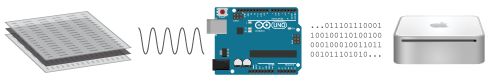
\includegraphics[width=0.9\linewidth]{figures/touch/process}
  \caption{Data process}
   \label{data-process}
\end{figure}

The top layer is made of 3 mm thick neoprene from an old mouse pad with one long conductive thread, made of stainless steel fibers, sewn into it.
Neoprene is easy to work with and gives a natural force-feedback when touched because of its thickness, but lacks the naturalness of normal fabric used for clothing.
The middle layer is made from anti-static polymer bags that are normally used to protect electronics. 
Some types of anti-static bags, such as the ones we have used, act as semi-conductors with piezoresistive capabilities and therefore fits in a FSR sensor.
We have tested three different types of anti-static bags, two transparent and one black, but only black ones are piezoresistive.
We do not know if this is the general case as we only had a limited number of samples.
The bottom layer is another layer of neoprene, but with separate conductive stitchings for each of the 2 x 3 cells.
The setup is illustrated in figure~\ref{layers_iteration1}.

\begin{figure}[t]
\centering
\begin{subfigure}[t]{.44\textwidth}
  \centering
  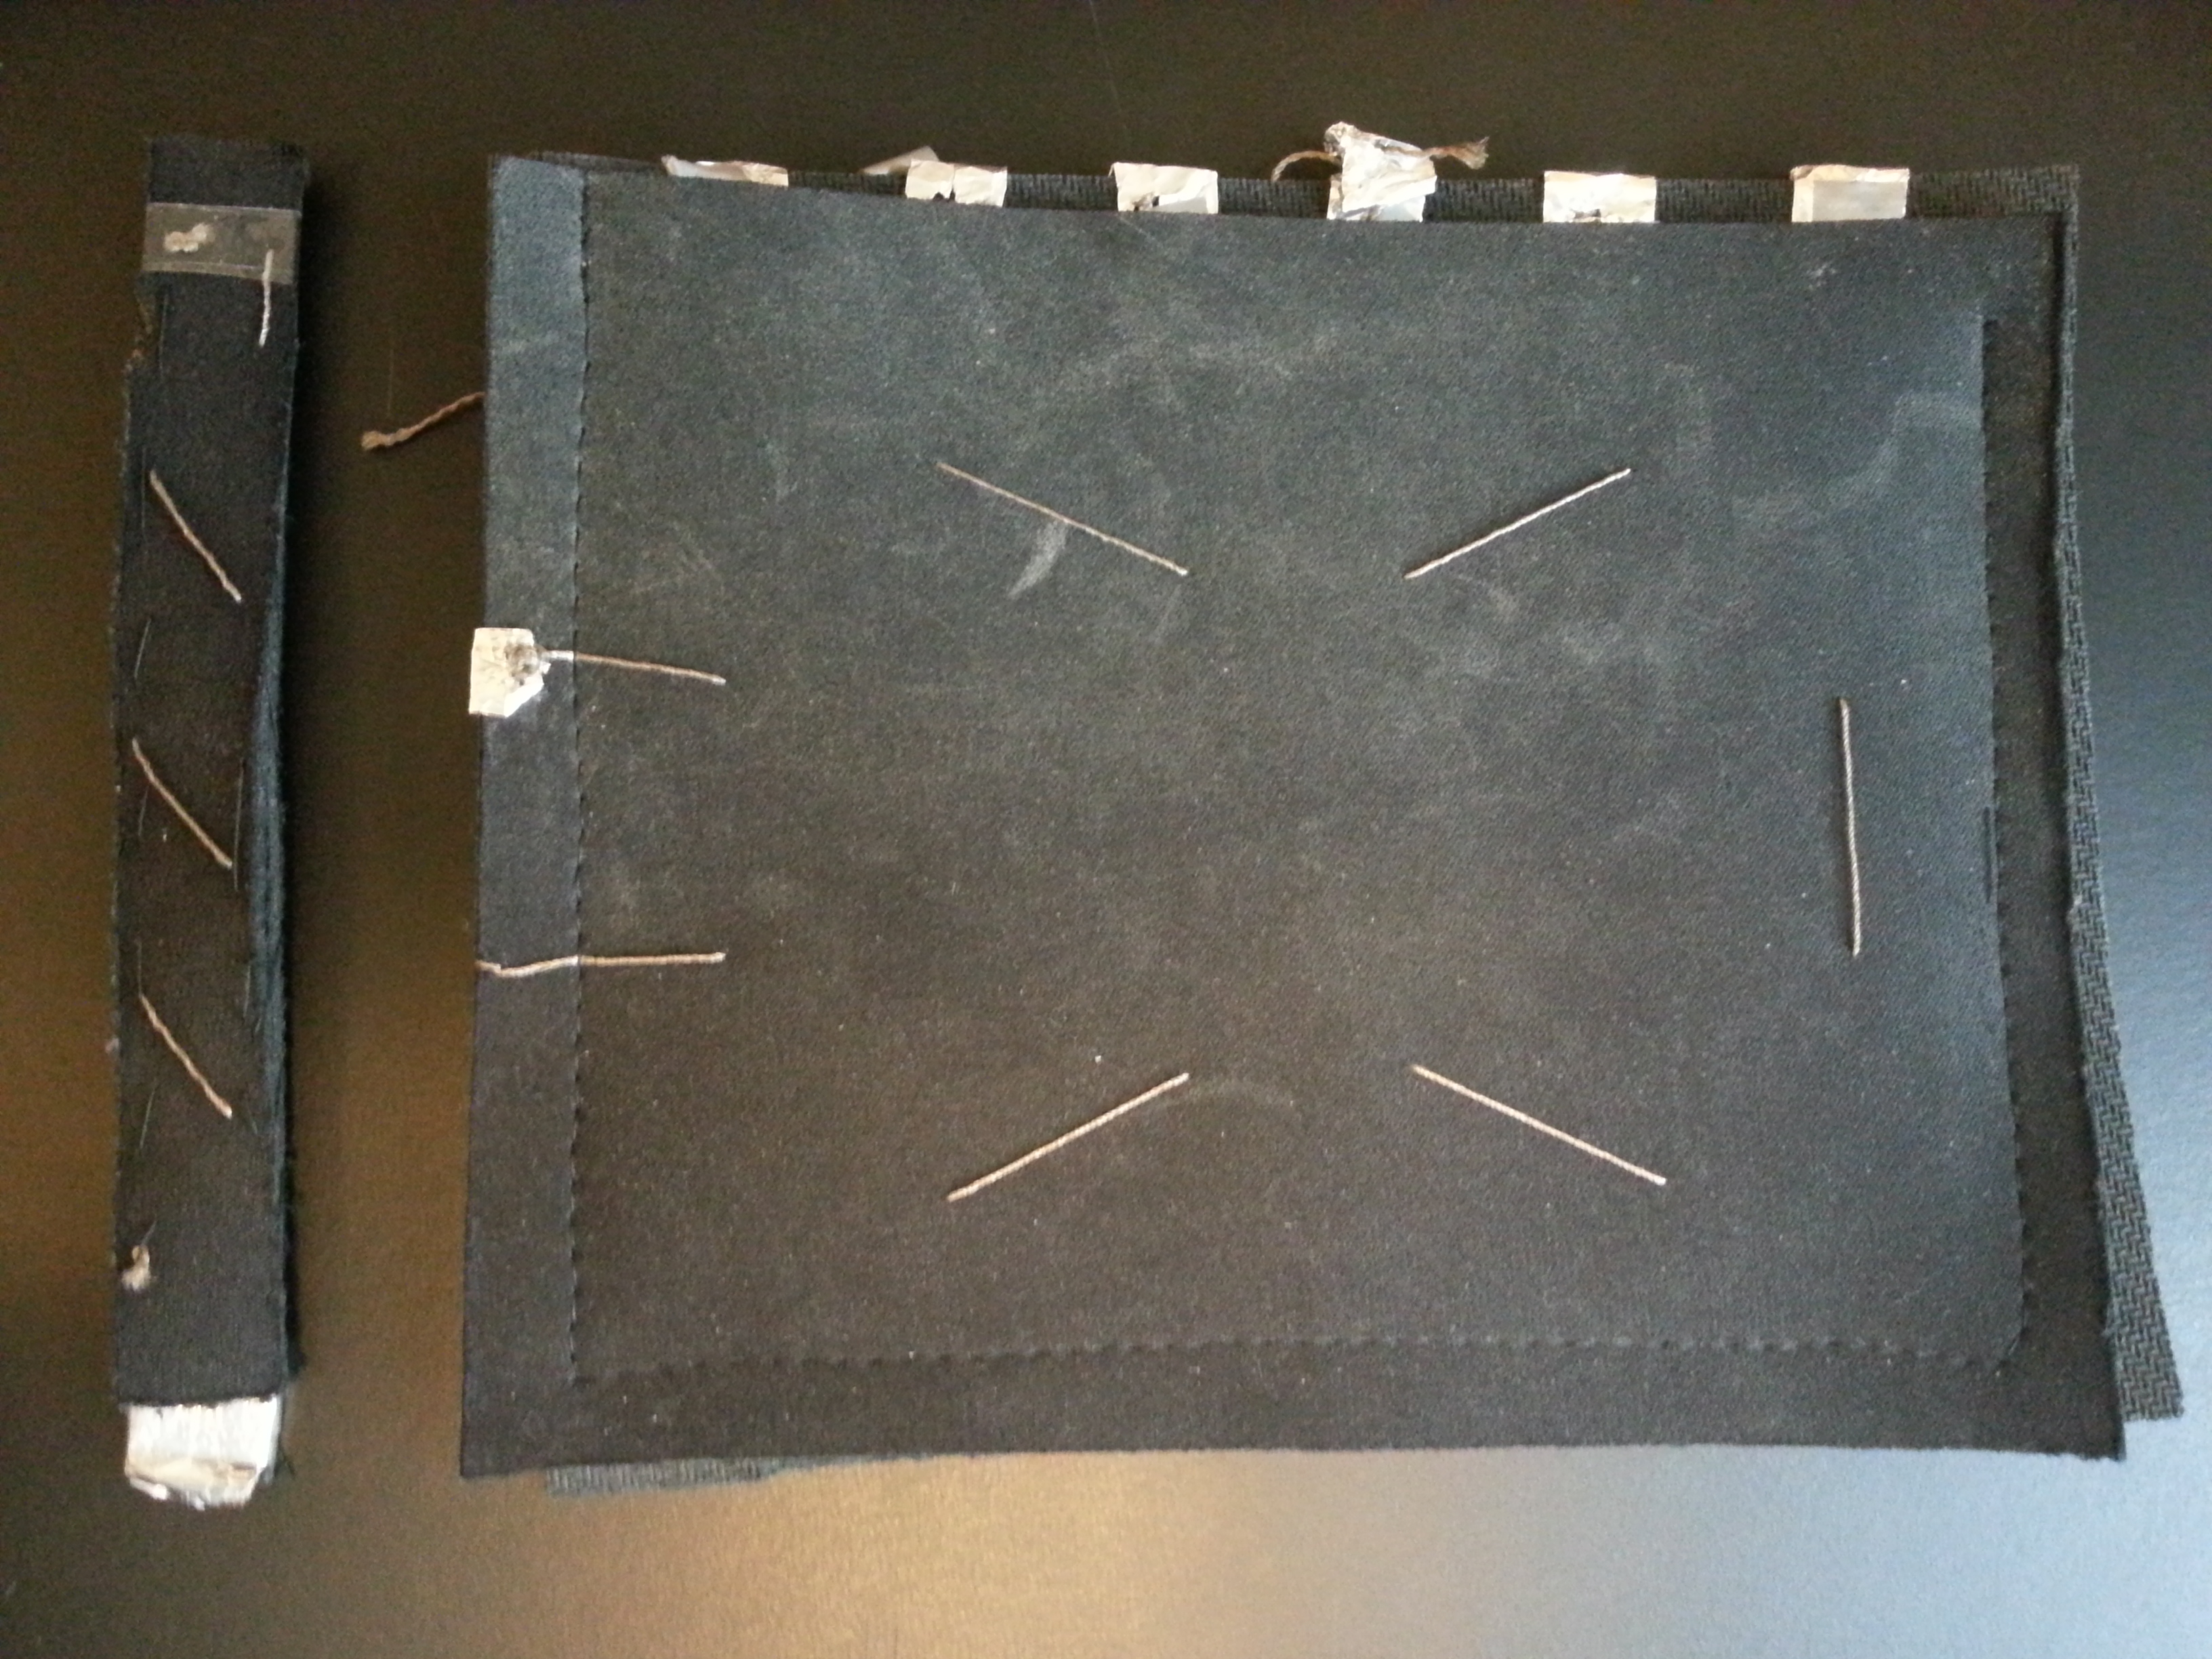
\includegraphics[width=\linewidth]{figures/touch/proto1_1}
  \caption{On the left is our simple bend sensor and on the right our 2x3 pressure matrix.}
\end{subfigure}%
\hspace{0.02\textwidth}
\begin{subfigure}[t]{.44\textwidth}
  \centering
  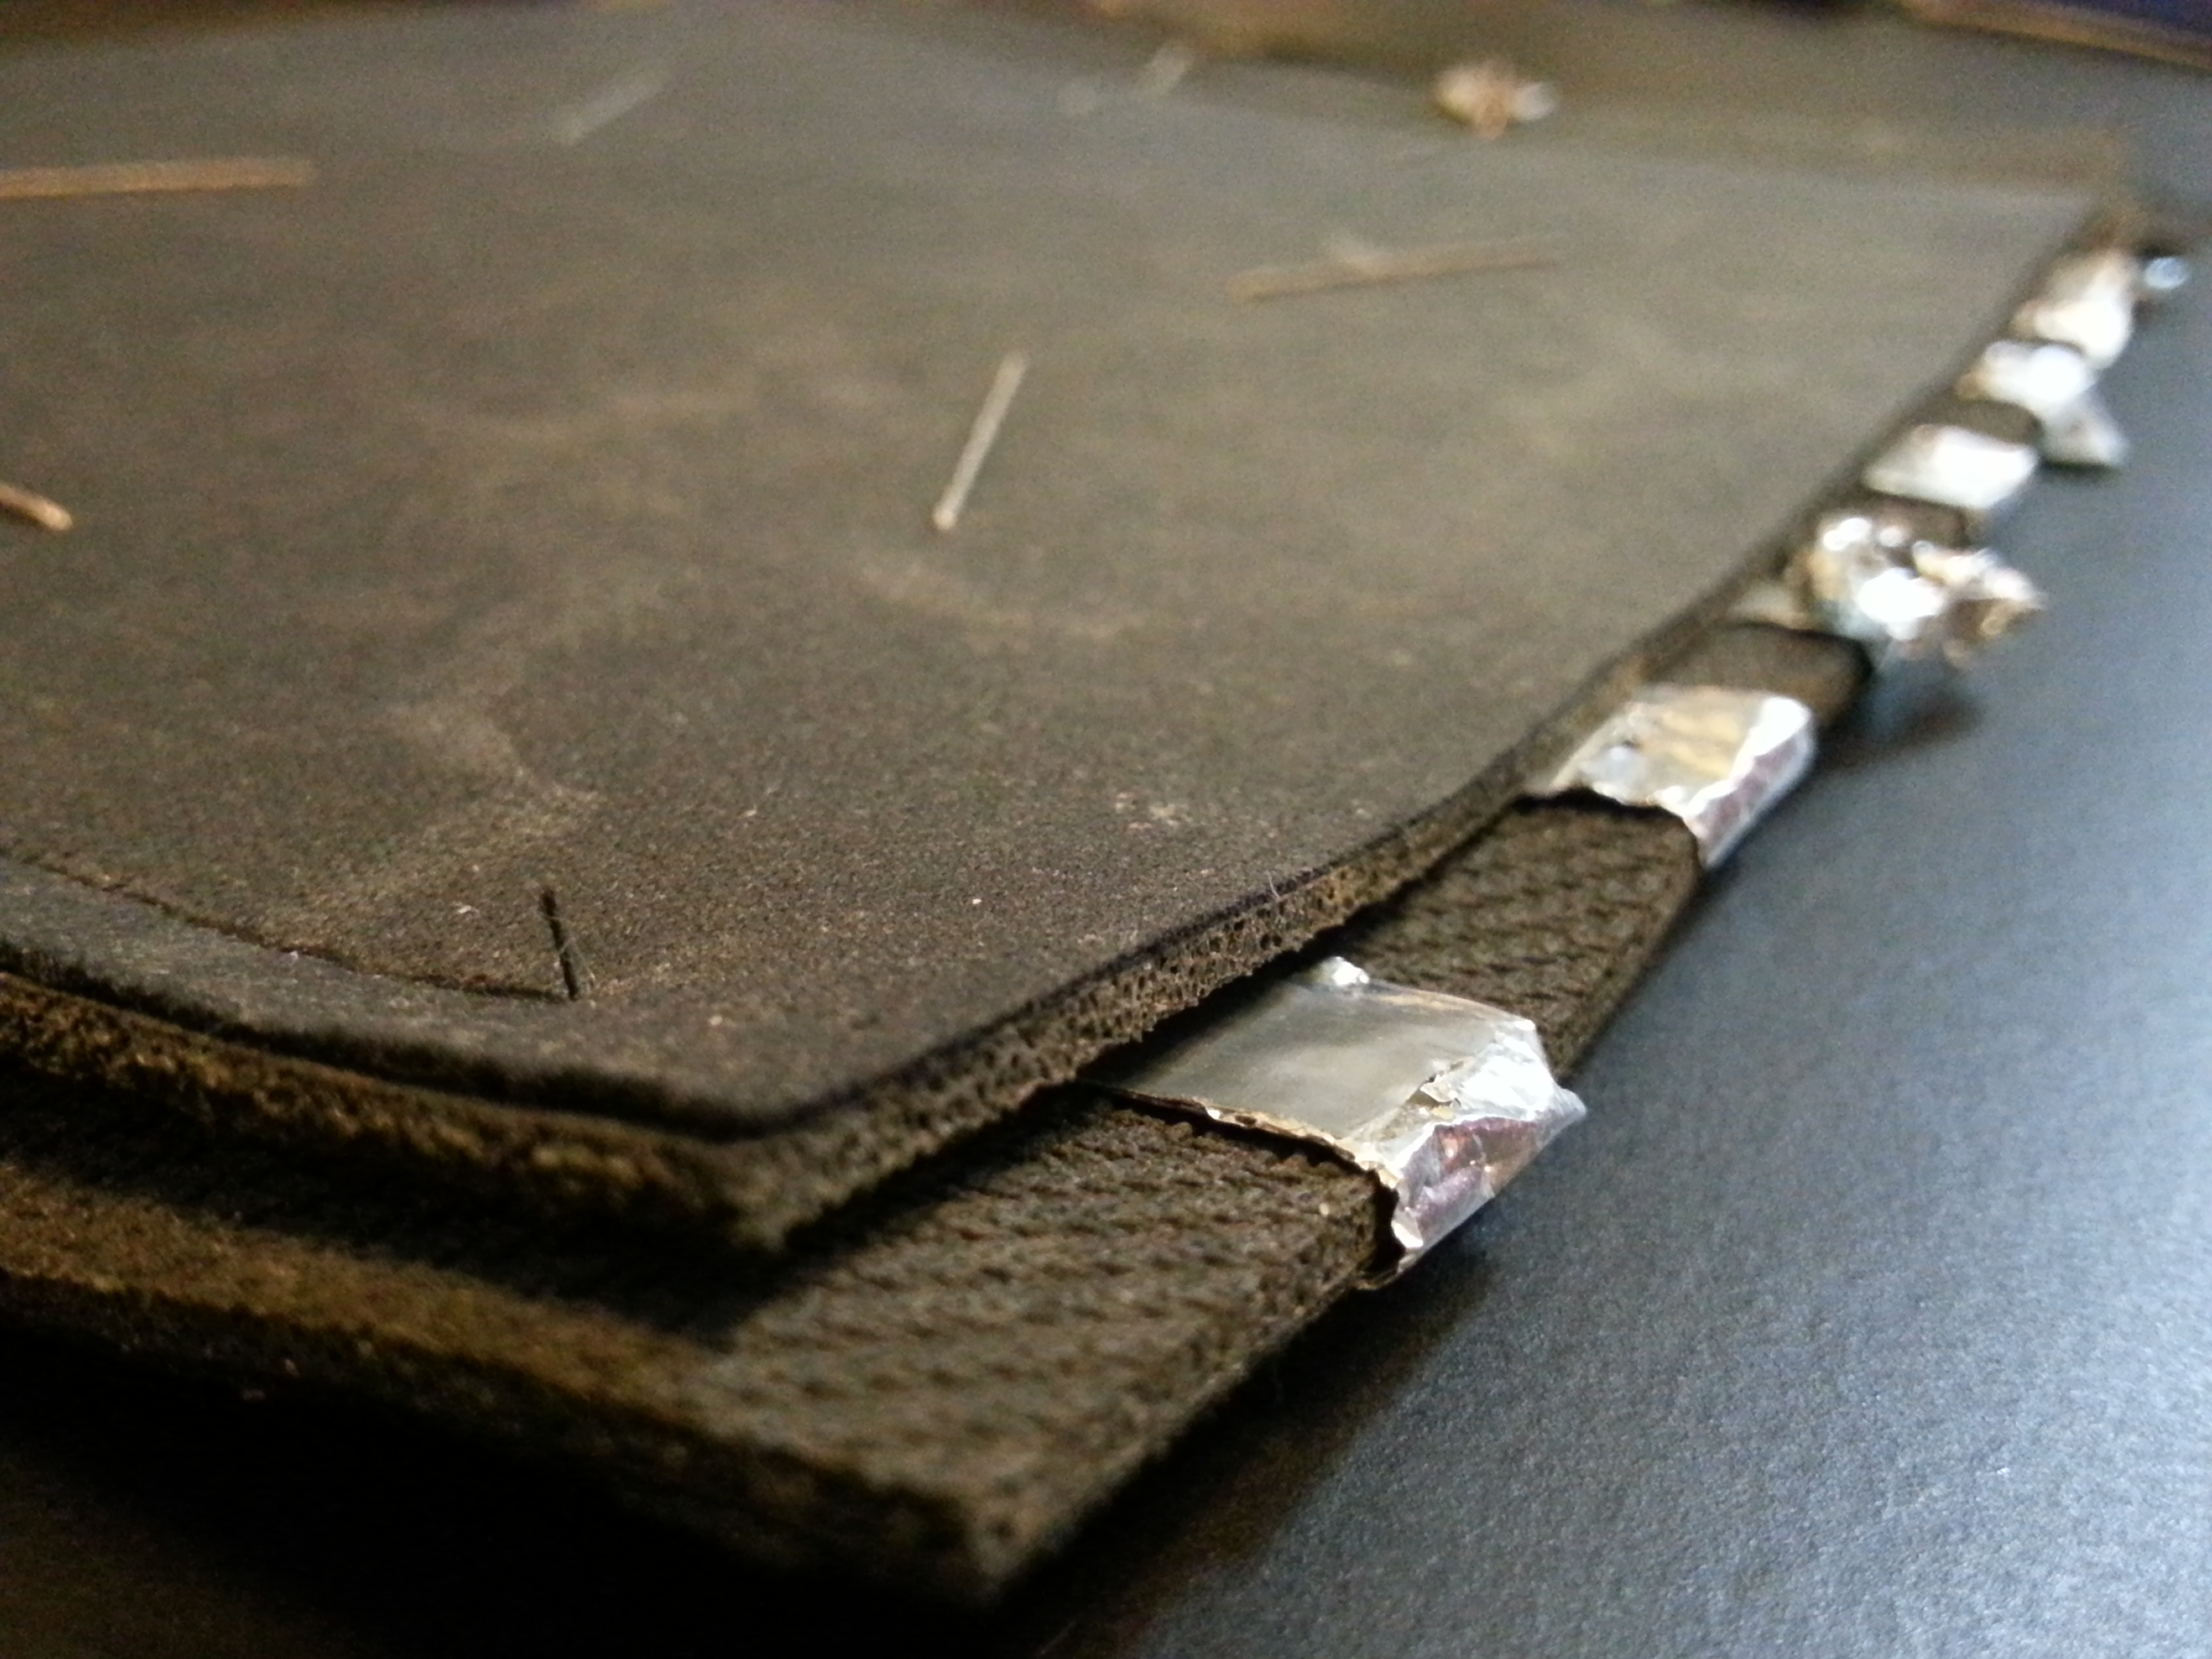
\includegraphics[width=\linewidth]{figures/touch/proto1_2}
  \caption{A close up of the materials.}
\end{subfigure}
\caption{First iteration of our touch prototype}
\label{prototype_1}
\end{figure}

\begin{figure}[b]
  \centering
  \begin{minipage}[b]{.8\textwidth}
    \centering
    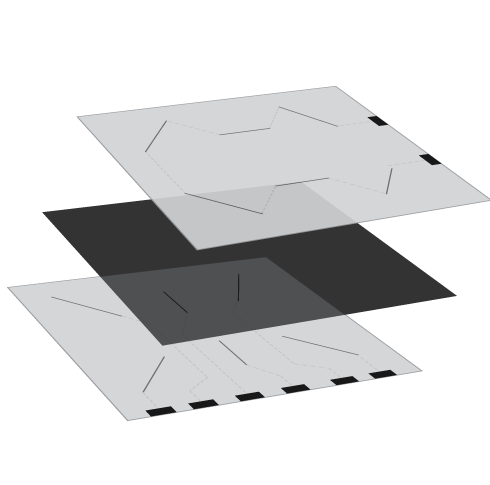
\includegraphics[width=.7\linewidth]{figures/touch/layers_it_1}
    \caption{The three layers of our touch sensitive fabric showing the construction principle of iteration 1.}
    \label{layers_iteration1}
  \end{minipage}
\end{figure}

By sending a 5V signal into the single top layer stitch, each of the six (\(2*3\)) bottom layer outputs can now be read on the Arduino after passing through the piezoresistive material.  
As pressure is applied to the different sections the voltage drop at the individual grid locations can now be measured with the analog input pins on the Arduino.
The ADC on the Arduino then translates the measured voltage, between 0--5V, into the amount of pressure that is applied to each of the cells, as a number between 0--1023.
The measured numbers will never reach the extremes as there is always some amount of resistance in the material.
A single layer of our anti-static bags has resistance values from around 180-200 KOhms, with little to no pressure applied, down to around 1.8 kOhms when pressed hard.
Depending on the piezoresistive material and the construction of the sensor, these values will vary.
\citet{rosenberg2009unmousepad} report values between 1.2 MOhms and 2.2 kOhms for their FSR ink.

Each of the cells acts in principle as a discrete sensor as they have their own individual output and are not influenced by each other.
This approach is simple, both in terms of Arduino setup and coding, and can attain the fastest possible update rates as no computation is needed to determine the location of the touch. 
The data received from the sensors are sent to Processing\footnote{The data visualisation program mentioned earlier} for visualisation as can be seen in figure~\ref{fig:ch:touch:it1:banana} where a the pressure of a banana is reflected in Processing running on the laptop.

\begin{figure}[h]
  \centering
  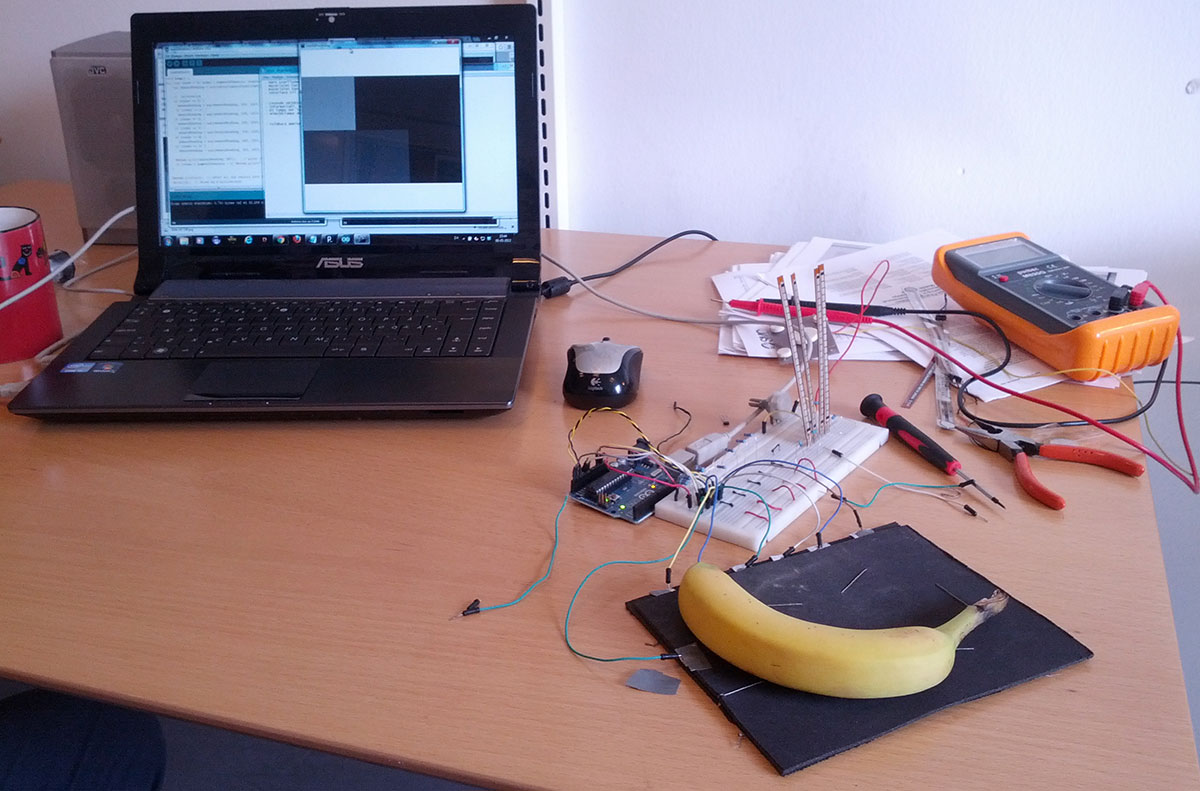
\includegraphics[width=.9\textwidth]{figures/touch/banana-processing}
  \caption{The prototype of iteration 1 tested with a banana.}
  \label{fig:ch:touch:it1:banana}
\end{figure}

\subsubsection{Iteration 1 discussion}
This quite simple prototype showed us that the basic principles for constructing a textile touch surface with the materials we have had access to, is indeed possible.
One of the major obstacles we found though was the transition from soft electronics (thread and anti-static bags) to hard electronics, as the conductive metal in the threads are woven into normal cotton thread, making soldering extremely hard.
For this first iteration we settled for a simple approach with glued on tin foil connectors as a quick-and-dirty solution.

A major disadvantage to making touch surfaces as a grid of discrete sensors, as we did in this iteration, is the lack of scalability.
There has to be an input pin for each cell in the touch grid you create, so for a given number of rows \(i\) and columns \(j\) you need hardware I/O pins equal to \(i*j\), which is not a suitable for normal micro-controllers which usually have 10--20 I/O pins.
So with this approach we would, just barely, be able to make a 4 x 4 grid with our Arduino Uno. 

\subsection{Iteration 2}
\label{ch:textiletouch:it2}
To combat the lack of scalability in iteration 1 we built a new version of the prototype.
To increase our touch surface resolution we improved the prototype in two ways, first by an improved construction and sewing approach inspired by rSkin (mentioned in \ref{ch:textiletouch:related:etextiles}) and secondly with interpolating post-processing of the input data inspired by \citep{rosenberg2009unmousepad}. 

\subsubsection{Construction principles}
For the second iteration we made a new 7 x 7 grid prototype, as seen in figure~\ref{prototype_2}, and instead of neoprene, we used sofa textile to get a more natural look and feel, and a larger degree of flexibility in the material.
We used the same basic three layer principle from iteration 1, but in order to solve the scalability issue the conductive thread is sewn in rows and columns as illustrated in figure~\ref{layers_iteration2_and_3}.
The principle is to first activate row 0, then read the output on each of the columns, then activate row 1 and read output on all columns, and so on, contentiously scanning the grid one row/column at a time.
To reduce the sensor noise non active rows and columns are connected to ground throughout the sweep.
Each finished sweep provide a pressure map that is sent to our applications.

\begin{figure}[h]
  \centering
  \begin{minipage}[b]{.8\textwidth}
    \centering
    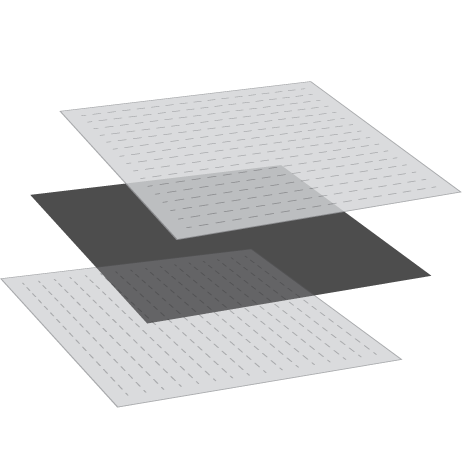
\includegraphics[width=.7\linewidth]{figures/touch/layers_it_23}
	\caption[The three layers of our touch sensitive fabric, iteration 2 and 3.]
   {The three layers of our touch sensitive fabric showing the construction principle of iteration 2 and 3.}
   \label{layers_iteration2_and_3}
   \end{minipage}
\end{figure}

As only one row and one column are active at a given time the micro-controller now only needs to have one I/O pin for input and one for output and can instead rely on multiplexers\footnote{http://en.wikipedia.org/wiki/Multiplexer} to shift the currently active row/column.
As a result the number of I/O pins now needed is dependent on the number of multiplexers that are used, greatly reducing the number needed for larger grids.

Generally for a multiplexer with \(2^n\) inputs, n control pins are needed plus one pin for the actual signal.
So for a \emph{j} x \emph{i} grid, the amount of pins needed would be \(\sqrt{j*i}\), compared to the \(i*j\) from iteration 1, reducing the amount of I/Os needed by the square root.

As mentioned earlier, if pressure is applied to the piezoresistive material the resistance decreases.
So if the fabric is bend or deformed in any way, this will happen, as the deformation puts stress on the material.
To allow the fabric to be bendable while attaining sensitivity we added a function to `reset' the pressure map by taking a snapshot of the pressure map in its bended state and use this snapshot to subtract from the active pressure map output.

\begin{figure}[h]
\centering
\begin{subfigure}[t]{.44\textwidth}
  \centering
  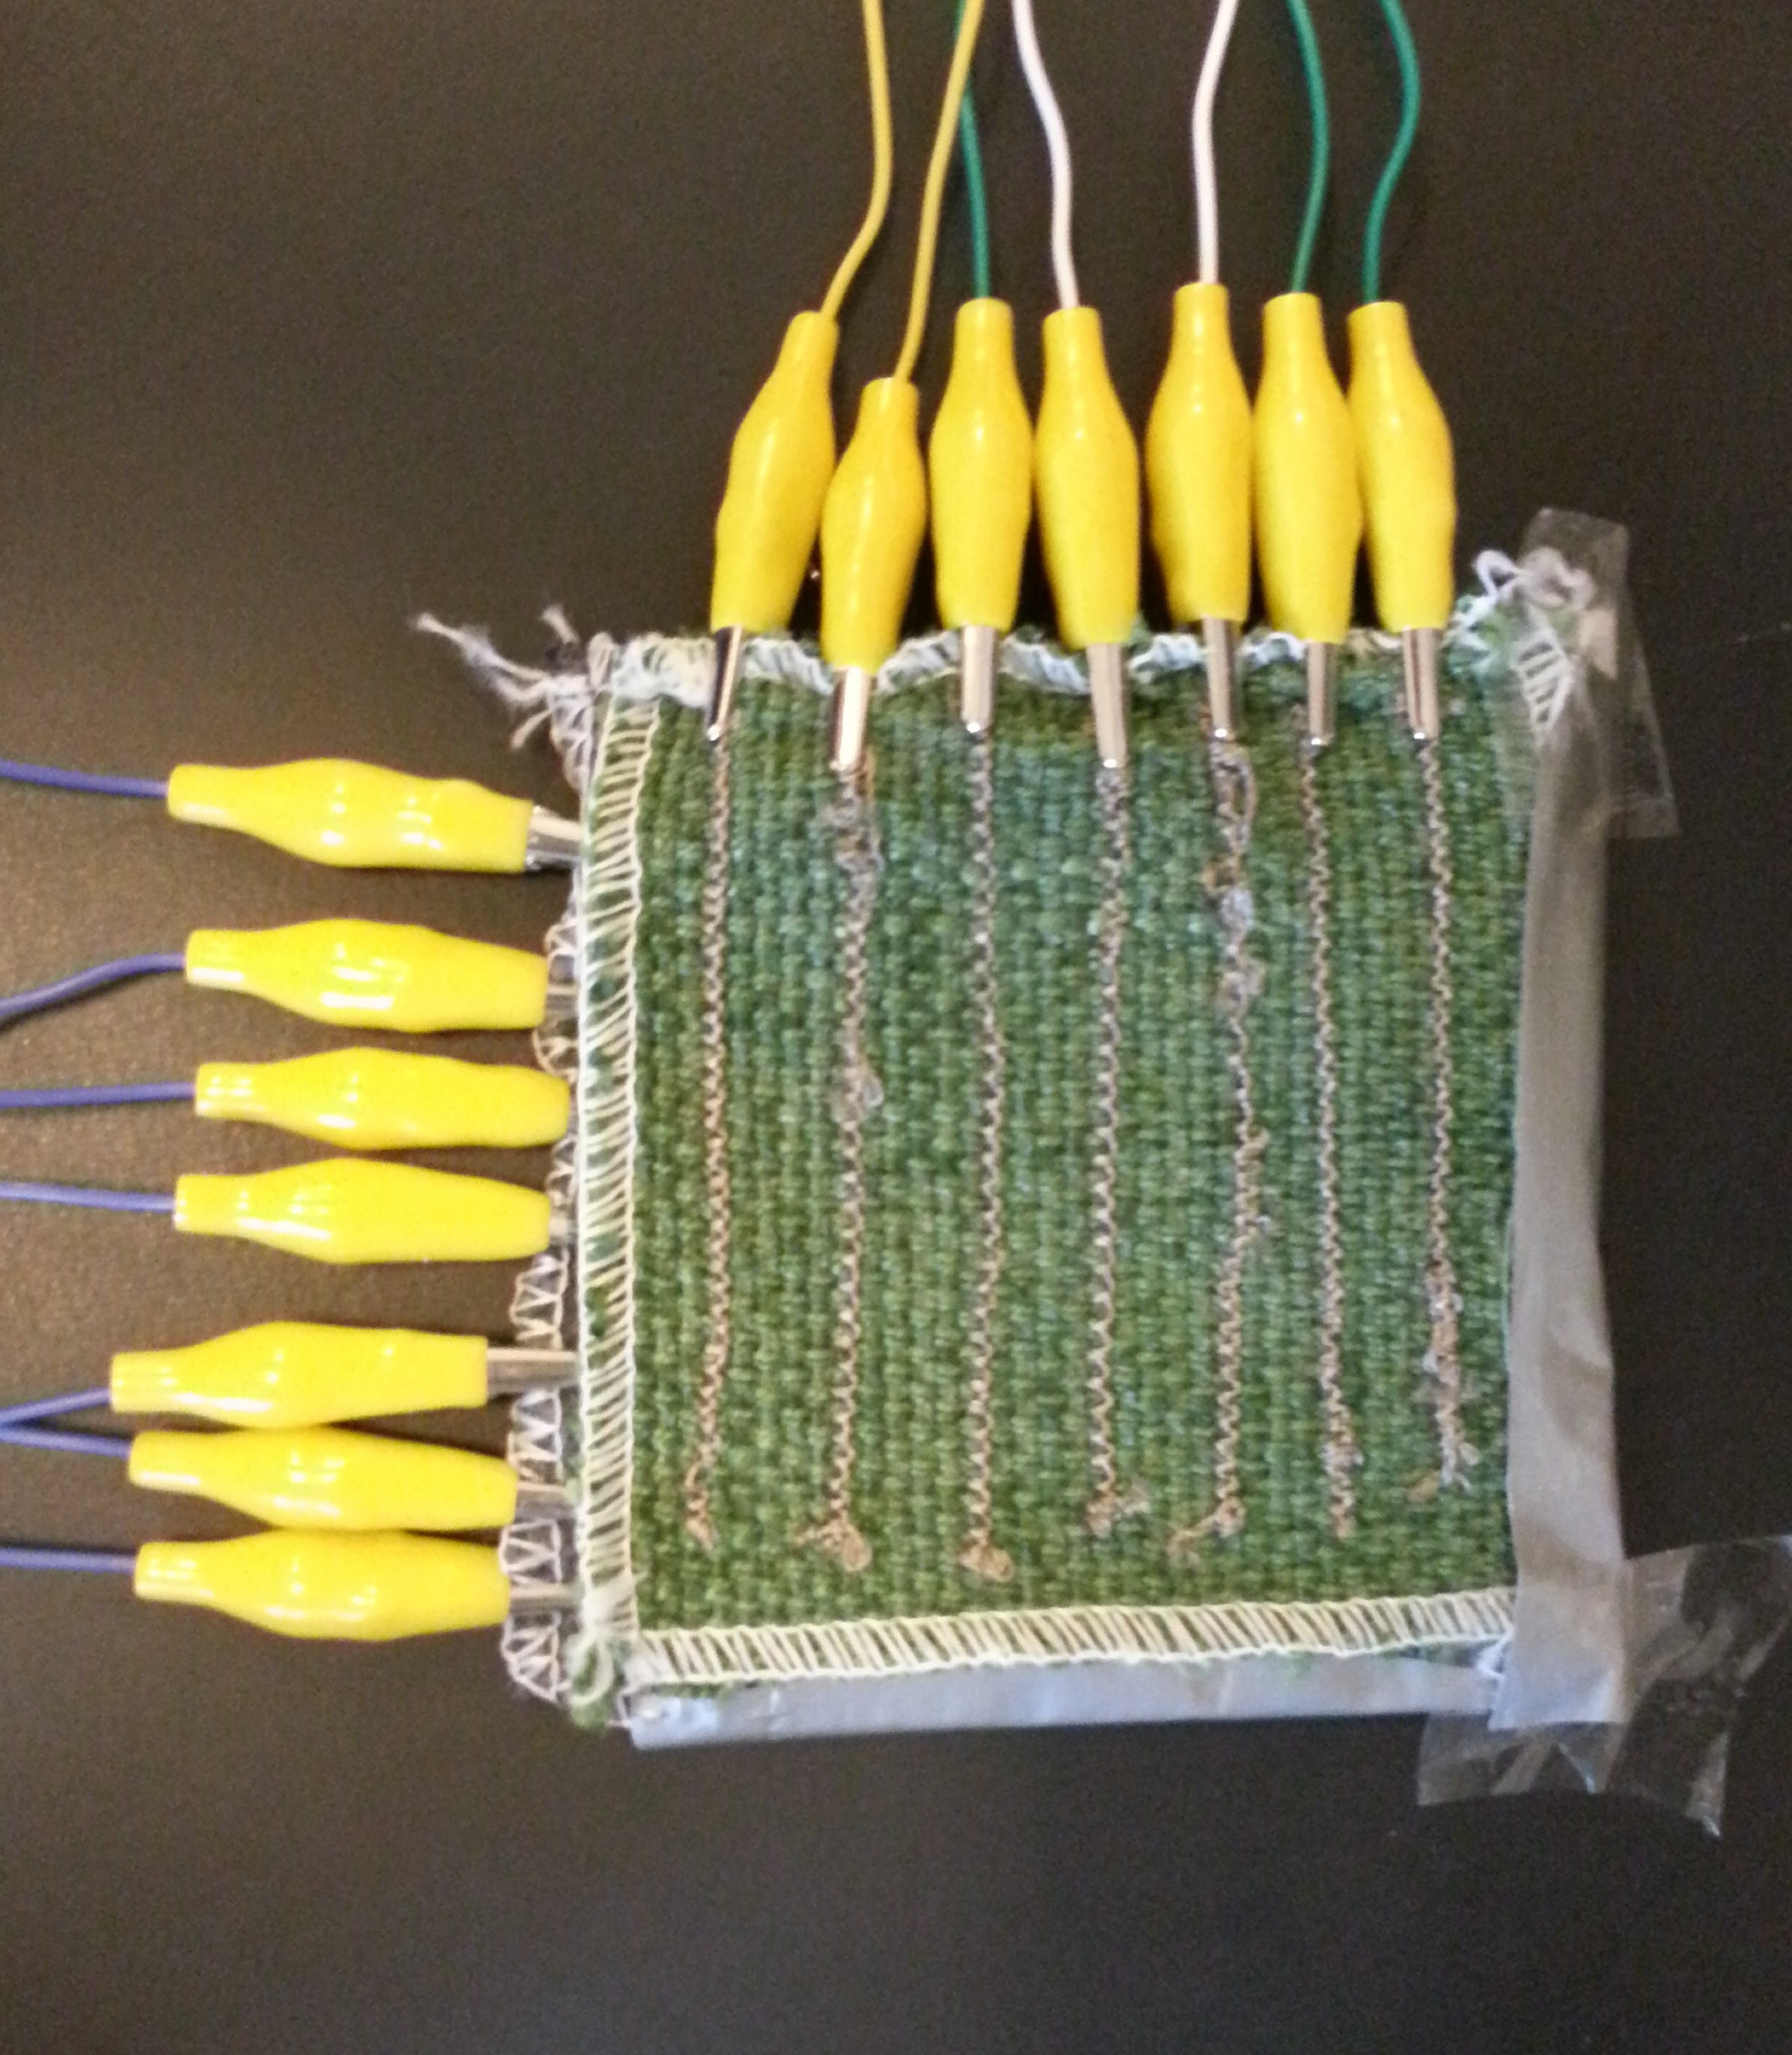
\includegraphics[width=\linewidth]{figures/touch/proto2_1}
\end{subfigure}%
\hspace{0.02\textwidth}
\begin{subfigure}[t]{.44\textwidth}
  \centering
  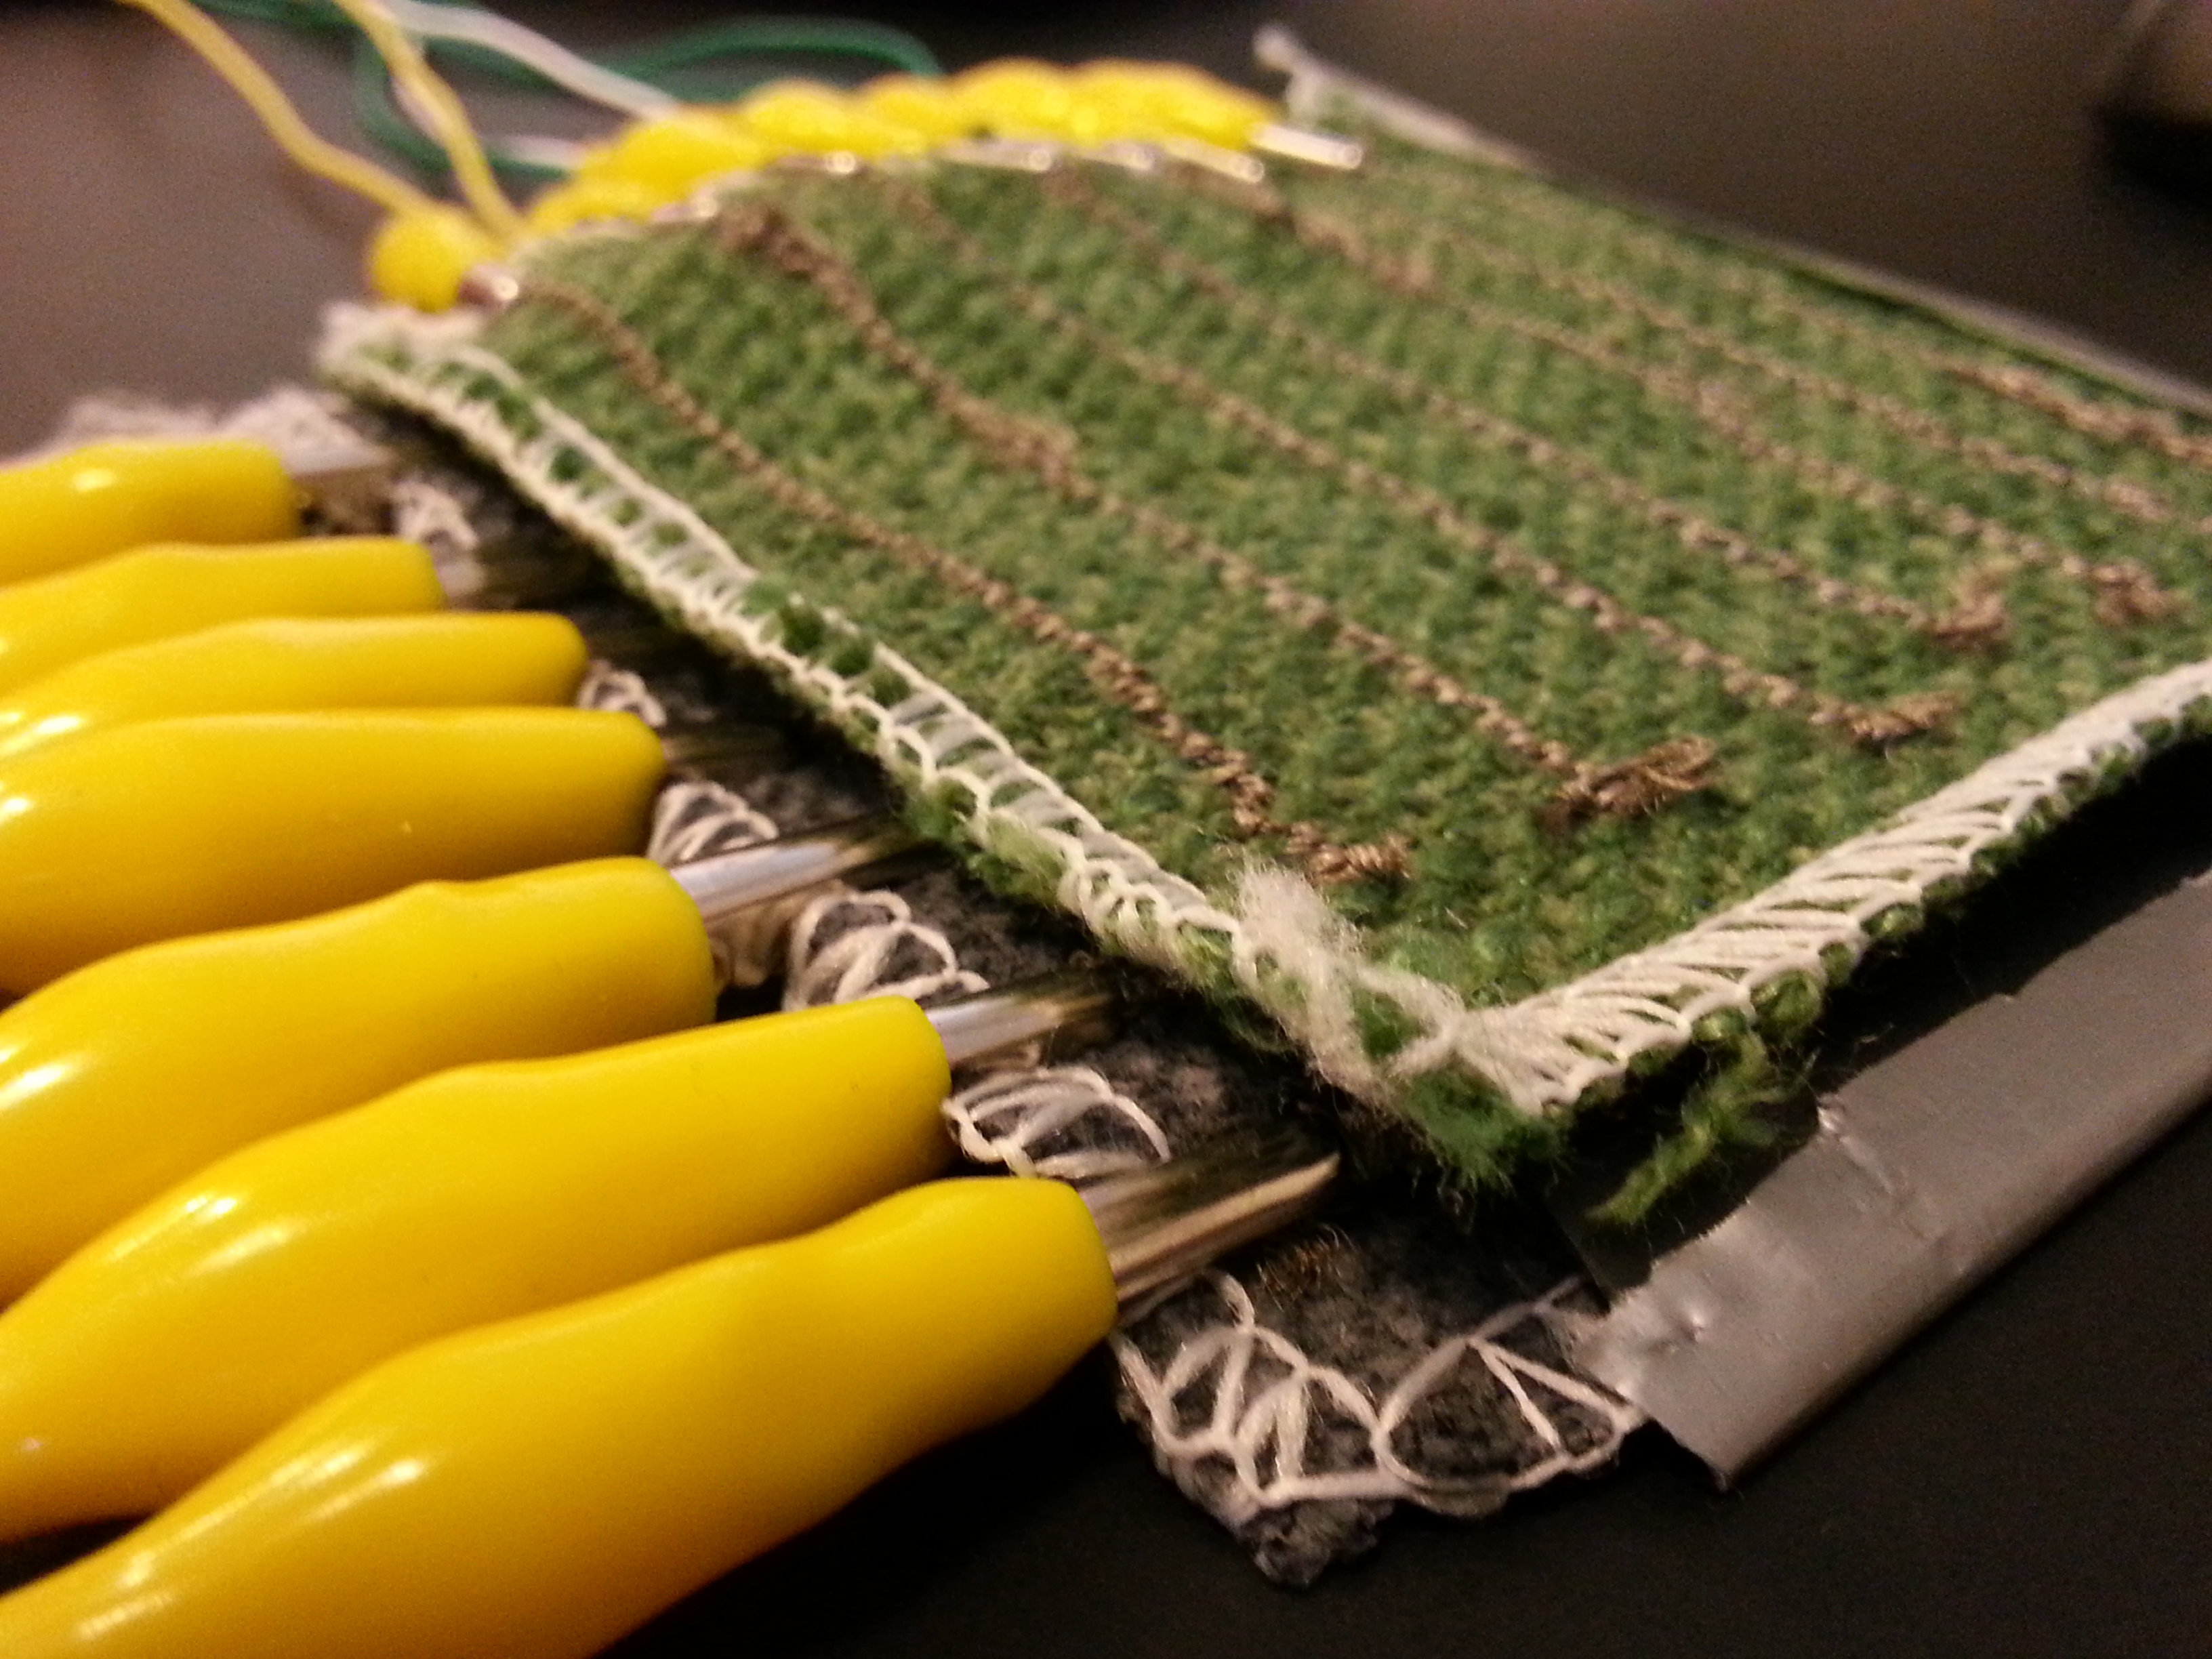
\includegraphics[width=\linewidth]{figures/touch/proto2_2}
\end{subfigure}
\caption{Second iteration of the prototype. The interactive area is a 7 x 7 grid with each row and column spaced approximately 1 cm apart from each other.}
\label{prototype_2}
\end{figure}

We now have a 7 x 7 grid fabric pad which in it self gives us a resolution of 49 cells compared to the 6 from iteration 1.
To increase this even further we now go from hardware to software.

\subsubsection{Peak detection and interpolating FSR}
\label{ch:textiletouch:it2-ifsr}
If a touch is made between two rows or columns our current approach will register the touch at the closest row/column intersection instead of the true position.
To improve on this aspect, \citet{rosenberg2009unmousepad} present a new approach to making FRS sensors called IFSR, or Interpolating Force Sensitive Resistance, in their UnMousePad project. The basic principle is to utilize that each sensor cell has overlapping regions of sensitivity with its neighbours.
This overlapping sensitivity is due to the fact that pressure at some position would also affect the surrounding neighbours as they are connected through the resistive middle layer.
This causes a spatial drop-off in sensitivity at the surrounding neighbours that is near linear for both the X and Y axis.
The fact that it is linear on both axes allows for bilinear interpolation to determine the location of touches between the conductive row/column lines, effectively increasing the resolution. 

Compared to the UnMousePad, which uses printed conductors, our fabric approach is a lot less `perfect' in its construction precision.
At the same time the fabric can bend and twist a lot more than a sheet of polymer, all in all generating a less precise pressure map which translates into less precise interpolation.
As a result we have taken a slightly more simple approach to the interpolation than \citet{rosenberg2009unmousepad} and in turn sacrificed some of the possible resolution gain.
\blank
For a given touch we first find the max value of the nearest intersection of the touch, point \(P_{max}\).
Because a touch gives a radial spread of current around itself, the precise location of the touch will always be in the region of the \(P_{max}\).
As there is a linear drop-off we can now take the readings from the surrounding \((X_{max}\pm1,Y_{max}\pm1))\) and use them to do a weighted average on both axes to approximate the correct position.
The new approximated point \(P_{approx}\) will, as a result of the radial spread, have a higher weight than the sensed \(P_{max}\) so we scale the value of \(P_{approx}\) with a factor according to the Euclidean distance to \(P_{max}\). 
The result of the interpolation is an approximated point which gives a more precise location of the touch than can be acquired directly from the raw sensor data.
We have illustrated the interpolation process in figure~\ref{fig:ch:touch:interpolation}.

\begin{figure}[h]
\centering
\begin{subfigure}[t]{.44\textwidth}
  \centering
  
\includegraphics[width=\linewidth]{figures/touch/p_map}
  \caption{Visualization of the raw touch data, black indicate no pressure and white indicate high pressure.}
\end{subfigure}%
\hspace{0.02\textwidth}
\begin{subfigure}[t]{.44\textwidth}
  \centering
  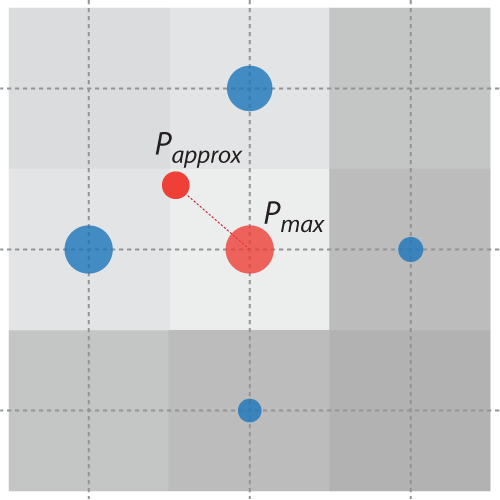
\includegraphics[width=\linewidth]{figures/touch/p_approximation}
  \caption{The weight-approximated position, based on the raw touch data from (a). The blue circles indicates the intensity of the values of the sensor cells surrounding the \(P_{max}\).}
\end{subfigure}
\caption{Illustration of the interpolation process.}
\label{fig:ch:touch:interpolation}
\end{figure}

\subsubsection{Iteration 2 discussion}
For this type of application where a large number of individual sensor cells are needed the construction approach we have used in this iteration is by far superior to the one from iteration 1.
It is a more complex setup both in software and hardware but it does in turn enable much larger sensor arrays than before as we showed before with the amount of I/O pins needed.
As it scales up it is of course more computational heavy on the Arduino CPU as the multiplexers and, in our case, 49 sensor cells need to be controlled, but as this is still only a 7 x 7 grid we did not experience performance problems.

The interpolation point approximation was, to some degree, a success as it enabled us to up-scale the resolution with a factor 5 with only few approximation errors, but when scaled with a factor 10, which was the goal, quite a few errors appeared.
Many of these errors are due to the sewing of the conductive thread as it, because of the close seams, protrudes a bit where the stitches are, which can be seen by looking at figure~\ref{prototype_2}.
Also the precision of the sewing, as it is not machine-accurate, eliminates some of the linearity that we base our interpolation on, creating errors in the raw data that are hard to even out in the software.

\subsection{Iteration 3}
\label{ch:textiletouch:it3}
The focus of iteration 3 was twofold.
First of all, we wanted a larger interactive area for touch input and for more realistic conditions in later evaluations.
Secondly, we wanted to get more reliable raw data from the sensor grid to use for gesture interaction.
As we were aware of the possibility of generating imprecise data, as we have discussed in the previous iterations, from physical deformation, construction imprecision, material variations and approximation errors, the second focus was to implement a basis for gesture recognition that would function under these constraints.

\subsubsection{Construction Principles}
We used the same setup for iteration 3 but scaled to a 16 x 16 grid, providing 256 sensor cells after software upscaling, compared to the 49 sensor cells in iteration 2.
The prototype was made in linen which is robust but a lot finer and thinner than the sofa textile and the conductive thread was sewed with less close seams to avoid some of the problems from iteration 2.
The prototype can be seen in figure~\ref{fig:ch:textiletouch:final_prototype} and the schematics for the final hardware setup as well as links to the software implementation can be found in appendix \ref{app:textile-touch}.

\begin{figure}[h]
  \centering
  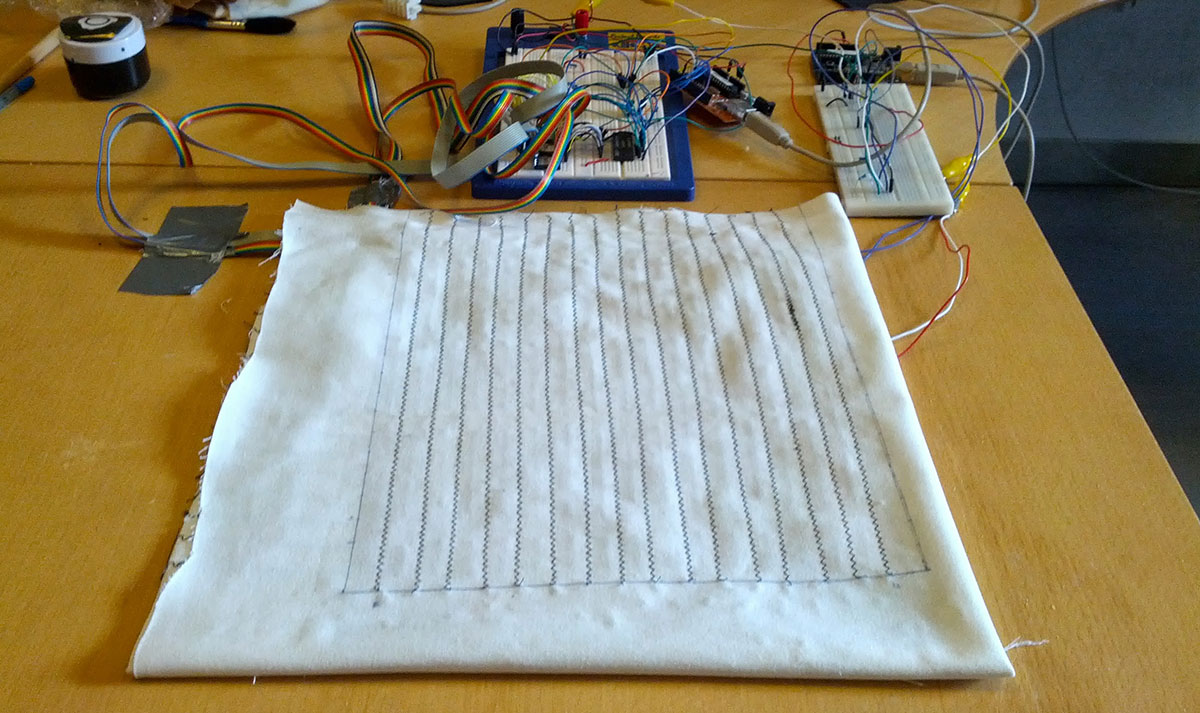
\includegraphics[width=.9\textwidth]{figures/touch/final_prototype}
  \caption{The final prototype.}
  \label{fig:ch:textiletouch:final_prototype}
\end{figure}

One of the main challenges in the construction of this iteration was the attachment of the wires to the conductive thread.
In iteration 1 we tried with glued on tin foil which only worked because we only had 6 connections to handle.
The 14 connections in iteration 2 were connected with alligator clips which, besides not looking elegant, tend to cause deformation of the fabric as they close upon it.
As we now had 32 connections to deal with we found that using ribbon cables would give a better structure.
Furthermore, as alligator clips were out of the question and as tin and textile do not work well together we needed to find an alternative for the connection.
Conductive paint turned out to be a good substitute and worked as a kind of ``cold''-soldering method - a secondary feature of the paint.
As the paint dries it functions like an adhesive but with the added ability of being conductive so you avoid the risk of the glue getting in between the two conductors severing the connection (see figure~\ref{fig:ch:textiletouch:barepaint}).

\begin{figure}[t]
\centering
\begin{subfigure}[t]{.44\textwidth}
  \centering
  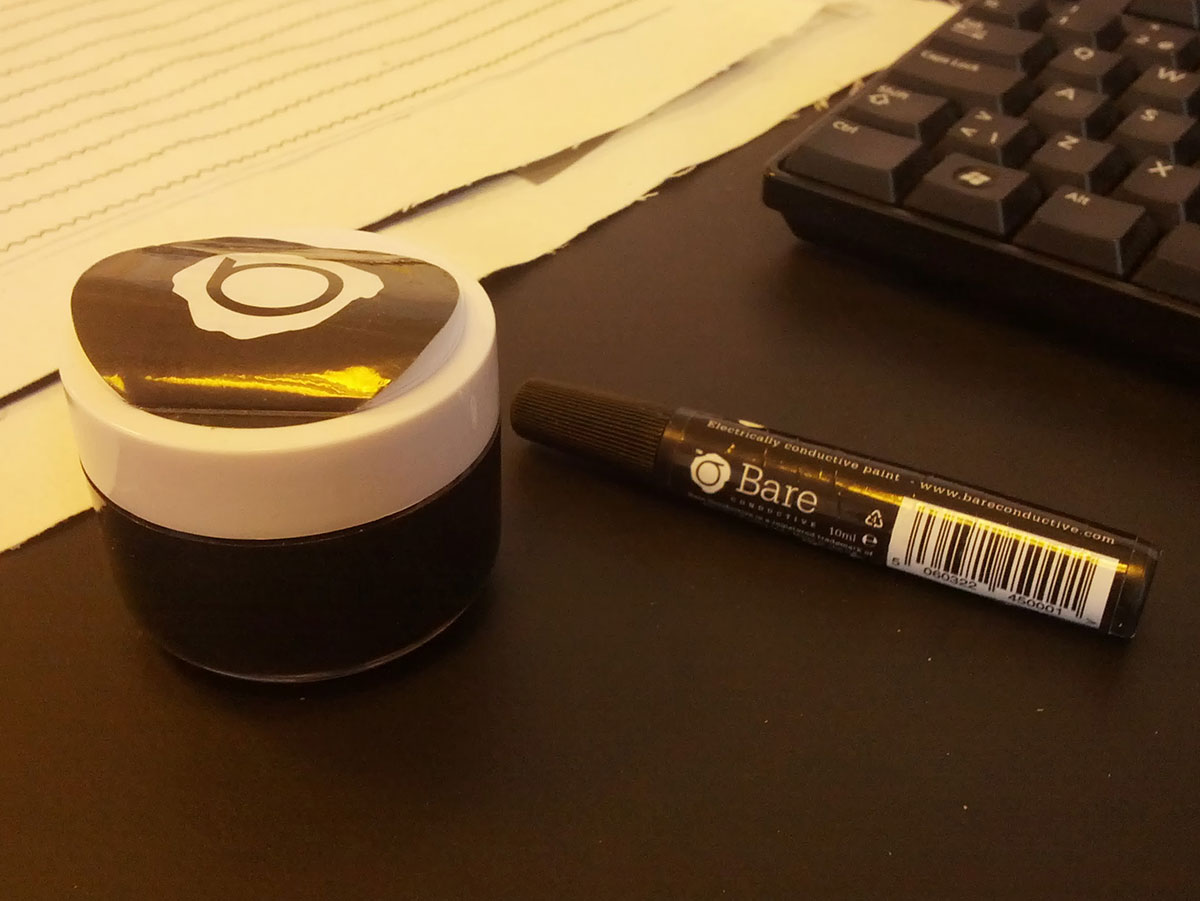
\includegraphics[width=\linewidth]{figures/touch/barepaint}
  \caption{Bare Paint, an electrically conductive ink, found at www.bareconductive.com}
\end{subfigure}%
\hspace{0.02\textwidth}
\begin{subfigure}[t]{.44\textwidth}
  \centering
  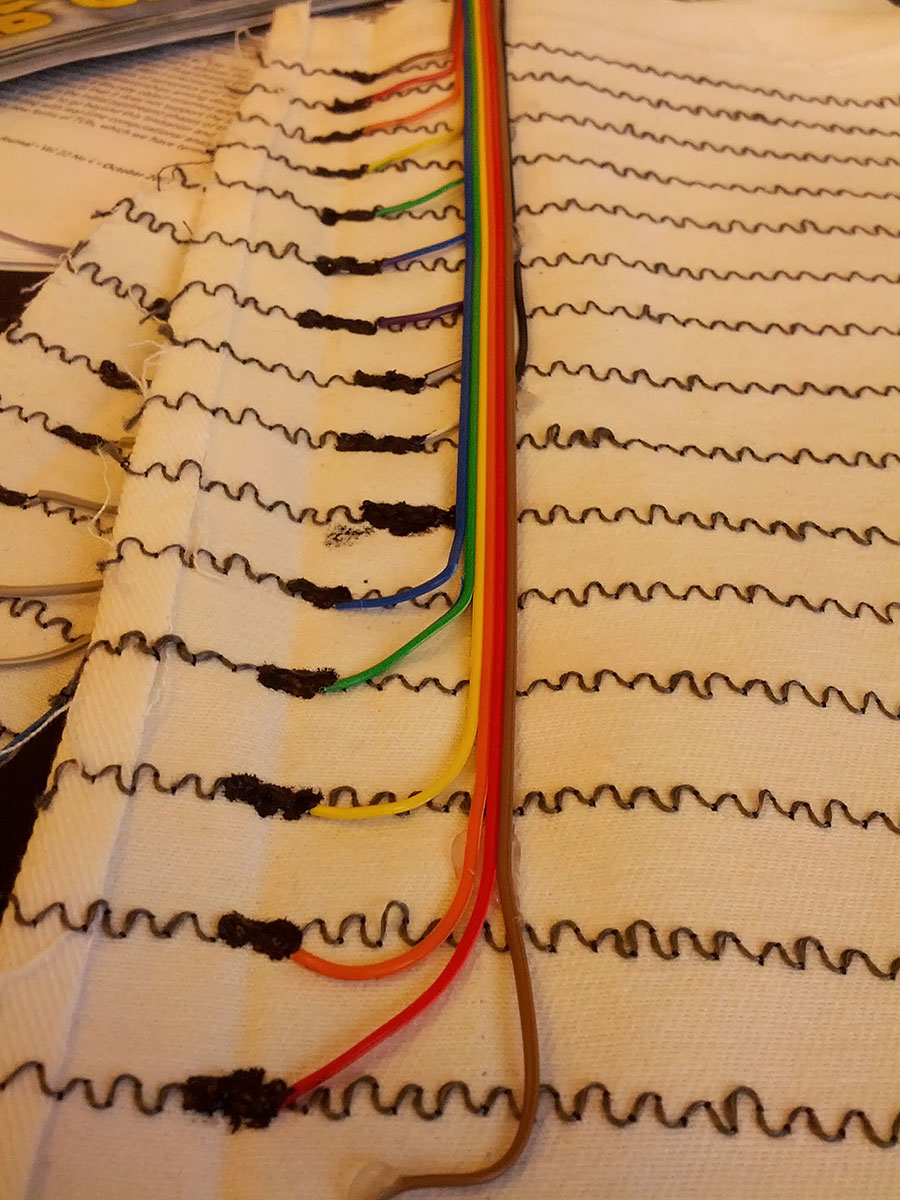
\includegraphics[width=\linewidth]{figures/touch/connectors}
  \caption{Bare Paint, used for ``cold''-soldering wires to conductive thread.}
\end{subfigure}
\caption{One solution for the challenge of connecting conductive thread to wires.}
\label{fig:ch:textiletouch:barepaint}
\end{figure}

\subsubsection{Data flow}
In figure~\ref{fig:textiletouch:dataflow} we illustrate each major step in the data flow and processing 
of our prototype.
The flow of data starts from sensor data in the \emph{physical layer} read by the Arduino.
Thereafter it is converted to digital data and streamed to the \emph{processing layer}.
In the \emph{processing layer} the data go through several filter stages for optimisation of the data.
Lastly the filtered data are delivered to the \emph{application layer} where data can be translated into gestures or visualisations.
We have already covered the principles of the physical layer in \ref{ch:textiletouch:it1} and peak detection and interpolation in \ref{ch:textiletouch:it2}.
Next we will cover some additional steps in the data flow and the \emph{application layer}.

\begin{figure}[b]
  \centering
      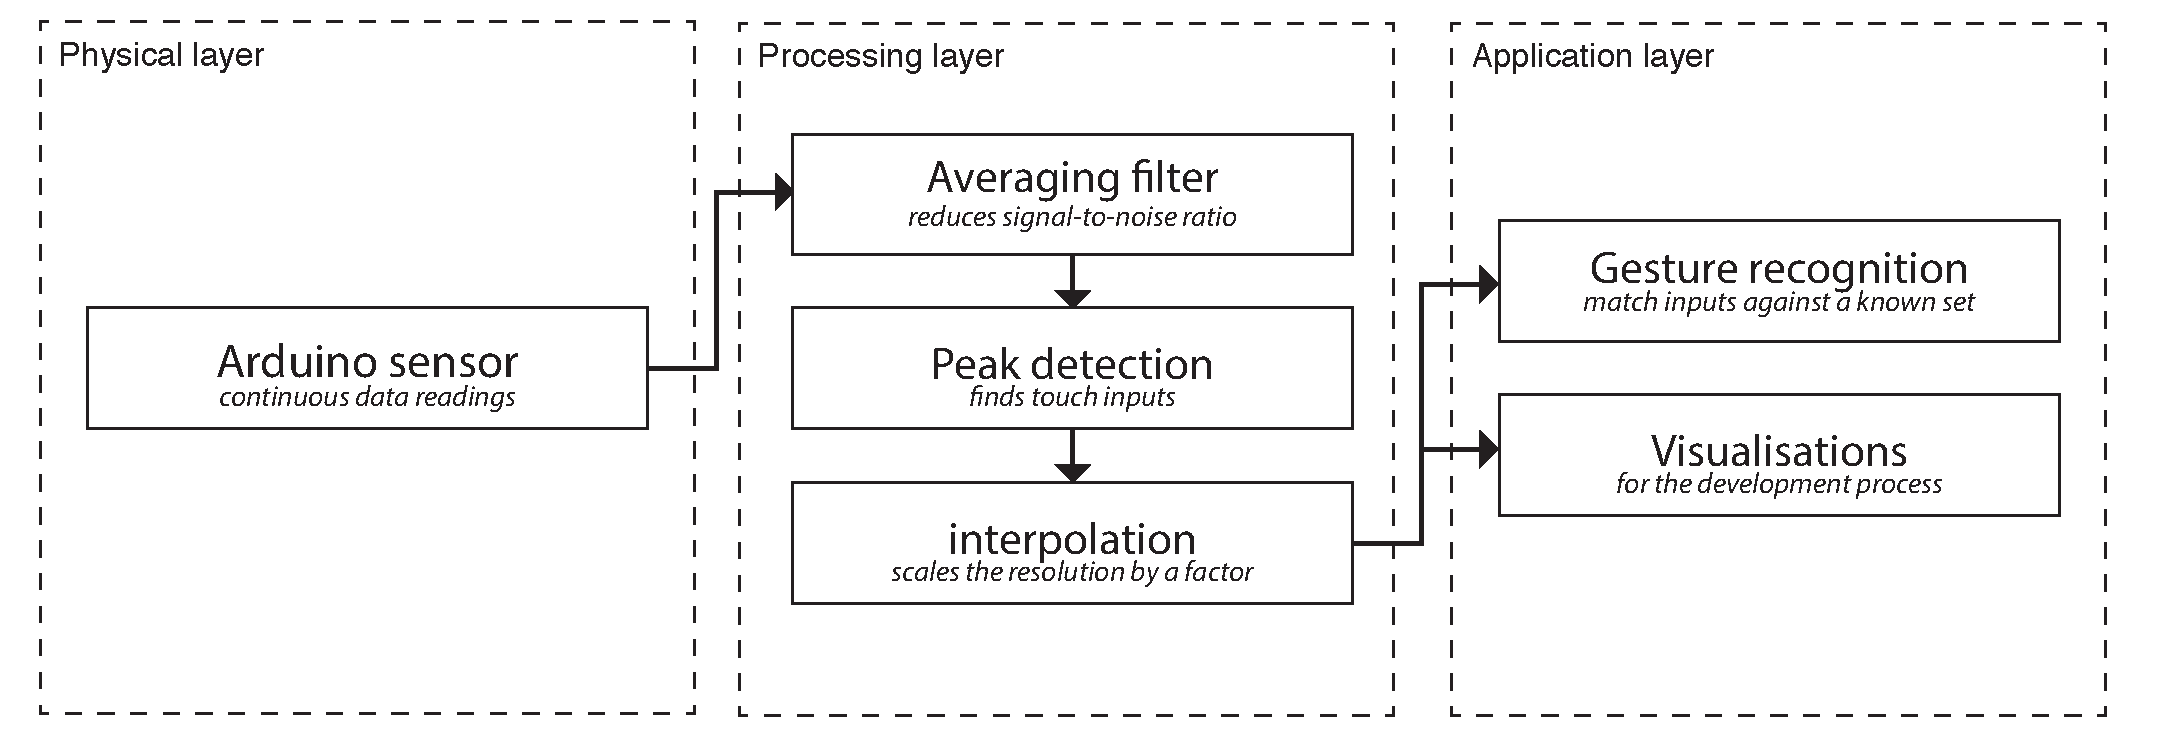
\includegraphics[width=.9\textwidth]{figures/touch/dataflow}
  \caption[The data flow from sensor to application.]
   {Textile Touch data flow from sensor to application.}
   \label{fig:textiletouch:dataflow}
\end{figure}

\subsubsection{Noise reduction}
On the software side we have implemented a simple averaging filter\footnote{http://en.wikipedia.org/wiki/Moving\_average} to reduce noise by increasing the signal-to-noise ratio, SNR.
This filter takes each input frame and averages the values of each cell with the cell values of \(x\) previous frames.
We have found that averaging over the past \(x = 2\) frames gives the best result for our setup. 
In this way noise such as sudden spikes will be reduced while preserving the actual touch values of the frame.

\subsubsection{Peak detection and interpolation}
The algorithm for detecting touch input and interpolation has generally not changed since iteration 2 (see~\nameref{ch:textiletouch:it2-ifsr} in \ref{ch:textiletouch:it2-ifsr}).

The new part is that we in iteration 3 also have introduced multi-touch input.
This is more a proof of concept feature which will not be fully functional and stable for interaction. The reason for this is that our code needs some adjustments to be able to provide proper stroke data to the recognition framework which would require too much implementation time.
So for now we can visualise multi-touch input and basic multi-touch drawing (see figure~\ref{fig:textiletouch:multitouch}).

An alternative would be to serve all recorded touch points to the \$N implementation, as opposed to \$P, but as noted earlier this would be unsatisfactory slow.

\begin{figure}[h]
  \centering
      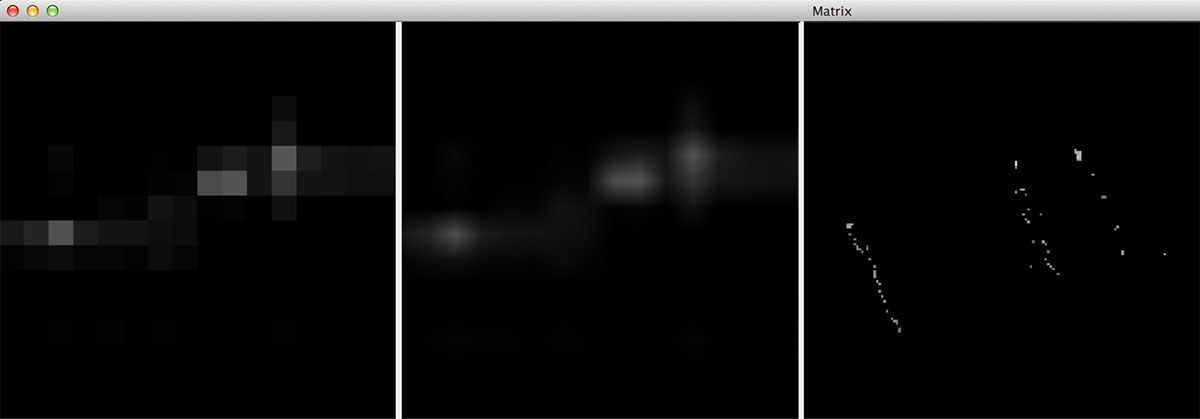
\includegraphics[width=.9\textwidth]{figures/touch/tt_multitouch}
  \caption{Multi-touch input visualised. 3 fingers are detected and 3 lines are drawn simultaneously.}
   \label{fig:textiletouch:multitouch}
\end{figure}

\subsubsection{Gesture recognition} 
\label{ch:textiletouch:gesture_implementation}

We have created an application that takes the filtered data of the \emph{processing layer} and abstracts it to a collection of strokes that are delivered to the \$P gesture recognition framework, which matches the input up against a set of predefined gestures templates.
Each of these predefined gestures map directly to a function in the application.
Our simple testing application is an audio and video application where functions such as channel/skip, volume, play, play pause and stop are implemented.
Furthermore, we have been experimenting with an extra layer of input for functions such as volume where the average touch force for the given gesture is calculated and used as a parameter for the amount of change.
In this way, the harder the touch pressure the more increase in volume.

The dollar family of recognisers were presented earlier in \ref{ch:textiletouch:gesture_recognition}.
Initially we experimented with the \$N implementation which was able to recognise gestures but with some limitations.
First of all, the recogniser was sensitive to the ordering of the strokes which meant that it could fail on the same gesture if drawn from a different starting point.
Secondly, there was a considerable amount of delay before a resulting gesture was found.
We measured this to be in the area of \(800\) to \(1000 ms\), a latency which in our opinion does influence the user experience.
This, we found out, is due to the complexity of the template matching in the \$N where the complexity is exponential to the number of strokes made in a gesture, as well as generally more complex algorithm than \$P.

After changing to the \$P implementation we got this delay down to \(< 10 ms\) which is quite an improvement.
This is because \$P avoids a combinatorial overhead of \$N where \$N matches up against every possible combination of stroke order and direction.
Furthermore, the \$P implementation does not distinguish the order of the strokes which allows for subjective ways of drawing specific shapes.

One limitation of both implementations is that they do not take in to account the orientation of the input. 
This means that, for example, for a line to be recognised in both a vertical, horizontal and diagonal version they all need to have a predefined template. 

Also common to both is the ease of adding and removing new gesture templates which is a great benefit for enabling users to generate their own individual gestures.

\subsubsection{Interaction feedback} 

For haptic feedback we have used a vibration motor mounted on the rear of the prototype.
We have tested different patterns of vibration as feedback to find a suitable feedback approach.
For instance having the motor vibrate shortly for a haptic sensation in response to a matched gesture input.
Also, using a firm press to activate the system with a subsequent short vibration on activation.
Besides this, we have also tested the motor continuously vibrating in response to a touch as an indication of a touch being recorded.
This continuous vibration seems promising, in our opinion, especially if it is divided in to small intervals of on/off pulsations.
We are aware that the current vibration motor is not powerful enough to propagate vibrations to the entire surface of our prototype but we believe it will suffice for our evaluation.
But we also interpret it as being a balance between motor power and material.
The ability to propagate vibration is also constrained by the choice of materials, and the linen (textile) we have used does not excel in this respect.
The ability is limited even further by the linen not being stretched out completely in our prototype.

For testing simple visual feedback on the prototype itself we have installed a single LED which comes up through the textile.
As a variation of the continuous vibration of the motor we have tested the LED in similar manner where it blinks as an indication of input.
Additionally, the LED will blink to indicate that it has stopped recording strokes and will instead find a matching gesture.

% \begin{figure}[t]
% \centering
% \begin{subfigure}[t]{.44\textwidth}
%   \centering
%   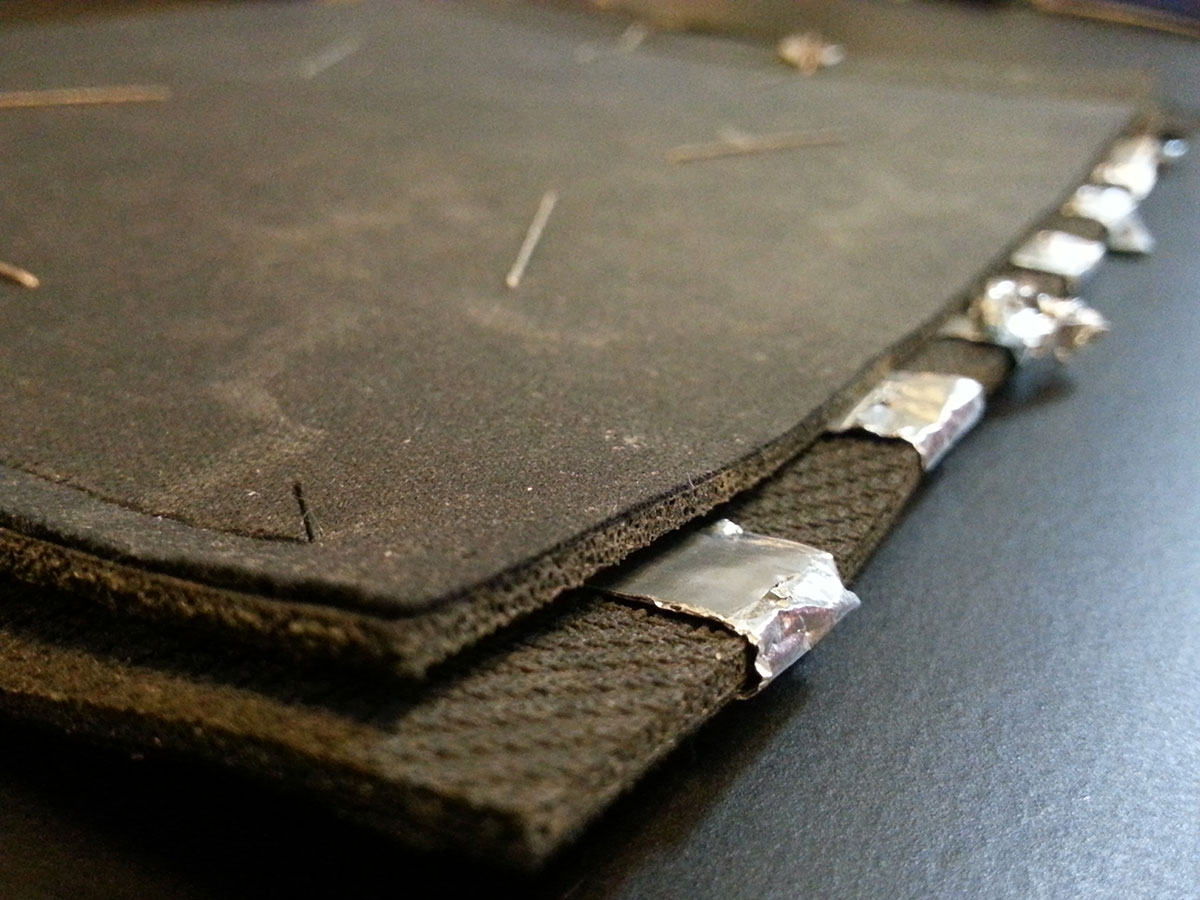
\includegraphics[width=.9\linewidth]{figures/touch/feedback_haptic}
%   \caption{A vibration motor mounted on the rear side of the prototype for haptic feedback.}
%   \label{fig:ch:textiletouch:feedback:haptic}
% \end{subfigure}%
% \hspace{0.02\textwidth}
% \begin{subfigure}[t]{.44\textwidth}
%   \centering
%   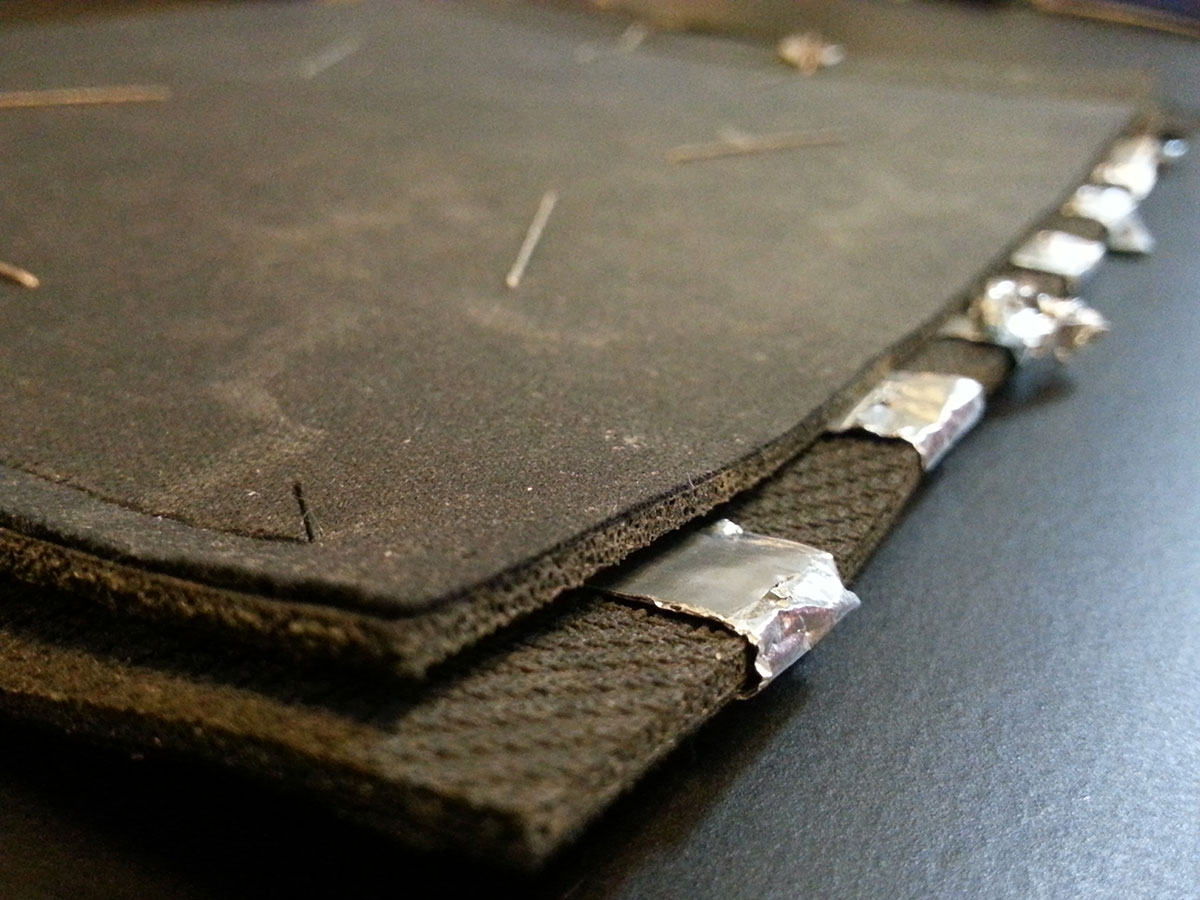
\includegraphics[width=.9\linewidth]{figures/touch/feedback_haptic}
%   \caption{A LED for visual feedback.}
%   \label{fig:ch:textiletouch:feedback:visual}
% \end{subfigure}
% \end{figure}

\subsubsection{Iteration 3 discussion} 

Although the 3rd iteration overcame some of the limitations of the 2nd iteration it still has some constraints that we would like to address.

One noticeable limitation is performance as foreseen in interation 2.
Our current Ardiuno Uno is not fast enough to always follow along with quick touch movements on the prototype.
Simple gestures like lines or simple characters are not affected as much as more complicated symbols.
A newer and exceedingly faster Arduino Due\footnote{http://arduino.cc/en/Main/ArduinoBoardDue}, an ARM-based board which operates at a clock speed of 84 MHz, has recently been released and would greatly outperform our older 8 MHz Arduino Uno.

One of the reasons for scaling up the prototype was to get a larger area for touch input.
In the process of tripling the dimensions of the prototype (from approximately \(8x8cm\) to \(25x25cm\)) we also increased the amount of rows and columns but with a little extra spacing (\(1.5cm\)) between the individual lines.
It seems that this spacing has become a bit too large, meaning that pressing in between the intersections of two rows and two columns does not propagate quite enough pressure to the surrounding line crossings, resulting in smaller pressure values (see figure~\ref{fig:textiletouch:intersections}).

We have tried to improve this in our approximation algorithm by multiplying the value with a factor relative to distance away from the line in both axes.
This has to some degree amended the issue but not fully.

\begin{figure}
\centering
\begin{minipage}[t]{.44\textwidth}
  \centering
  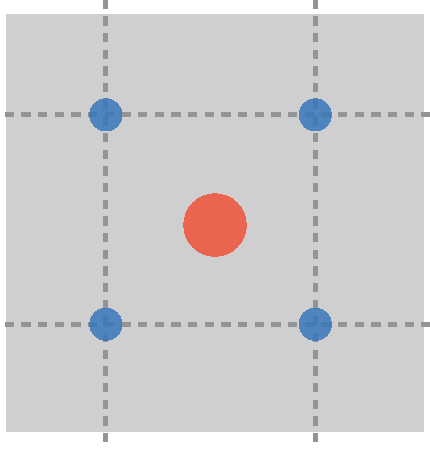
\includegraphics[width=\linewidth]{figures/touch/intersections}
  \caption[Pressing in between the intersection of two rows and two columns does not propagate enough pressure.]
  {Pressing in between the intersections of two rows and two columns (red dot) does not propagate enough pressure to the surrounding lines crossings (blue dots).}
  \label{fig:textiletouch:intersections}
\end{minipage}%
\hspace{0.02\textwidth}
\begin{minipage}[t]{.44\textwidth}
  \centering
  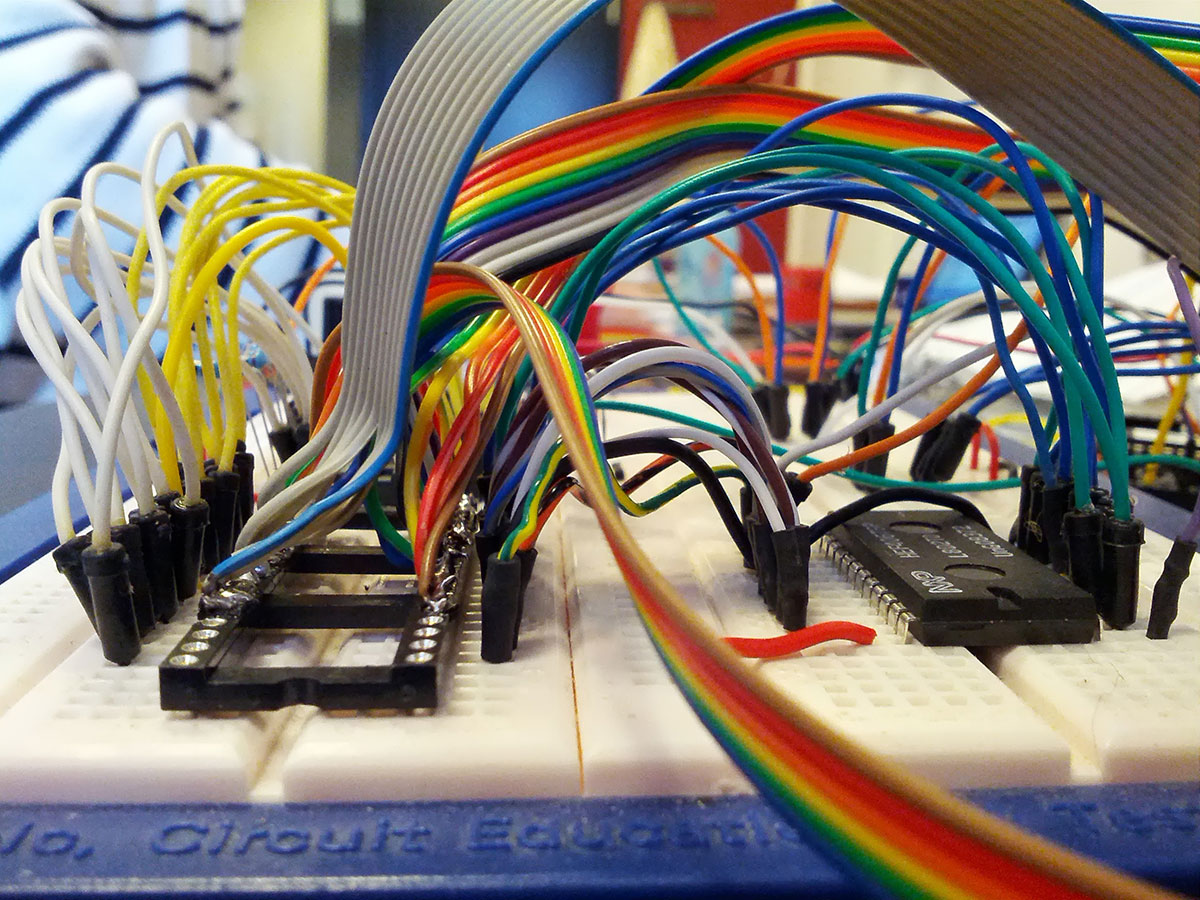
\includegraphics[width=\linewidth]{figures/touch/wires}
  \caption[Breadboard crowded with wires.]
  {Breadboard crowded with wires.}
  \label{fig:textiletouch:wires}
\end{minipage}
\end{figure}

An alternative approach is to reduce the spacing again to \(1cm\) or less but that would require quite a few extra wires which we already have quite a few of (see figure~\ref{fig:textiletouch:wires}).
Furthermore, increasing the grid resolution would result in an exponential growth in the amount of data to be transmitted by the micro controller.
With a \(16x16\) grid we are sending 256 values for every frame (\(10ms\)).
If we were to lower the spacing to \(1cm\) we would get a grid resolution of \(24x24\) which in turn would require a transmission of 576 values for every frame.
As our micro controller is already running at overcapacity this is out of the question for now, but by replacing the micro controller with a more powerful one, as mentioned before, increasing the resolution could become relevant again.
Therefore we see it as a balance between the size of the touch area and the complexity of the hardware setup.

Our exploration of possible interaction feedback has been limited, so further work on this would be appropriate.
We do envision that the application that is interacted with through the Textile Touch will provide some of the feedback, but more/better, both haptic and visual, feedback on the prototype could improve the user experience. 
